%%%%%%%%%%%%%%%%%%%%%%%%%%%%%%%%%%%%%%%%%%%%%%%%%%%%%%%%%%%%%%%%%%%%%%%%%%%%%%%
% Chapter 3: Procedimiento experimental
%%%%%%%%%%%%%%%%%%%%%%%%%%%%%%%%%%%%%%%%%%%%%%%%%%%%%%%%%%%%%%%%%%%%%%%%%%%%%%%

\leftline{\Large{\bf Introducci�n:}}
En �ste cap�tulo, se describir�n los diversos materiales utilizados en la elaboraci�n y ralizaci�n del algoritmo dise�ados en el software Python. Adem�s, se implementar� el algoritmo de la distribuci�n geom�trica, para observar los procesos en cada paso de ejecuci�n del programa. Finalmente, se expondr�n los resultados finales y las conclusiones que de ellos se desprendan.


%++++++++++++++++++++++++++++++++++++++++++++++++++++++++++++++++++++++++++++++
\section{Descripci�n de los experimentos}
\label{3:sec:1}

%ver el ejmplo del tri�ngulo.

%diagrama de flujo (Buscar el diagrama en latex)
\begin{enumerate}
	 \item \textbf{Distribuci�n Geometrica. }
\begin{description}
  \item[An�lisis:] Vease el cap�tulo 2.
  \item[Formulaci�n] Introducci�n de par�metros: Probabilidad $p$ y n�mero de casos $n$
  \item[Algoritmo: (ver Figura \ref{dflu}).]
\begin{figure}[h!]
  \centering
  % Requires \usepackage{graphicx}
  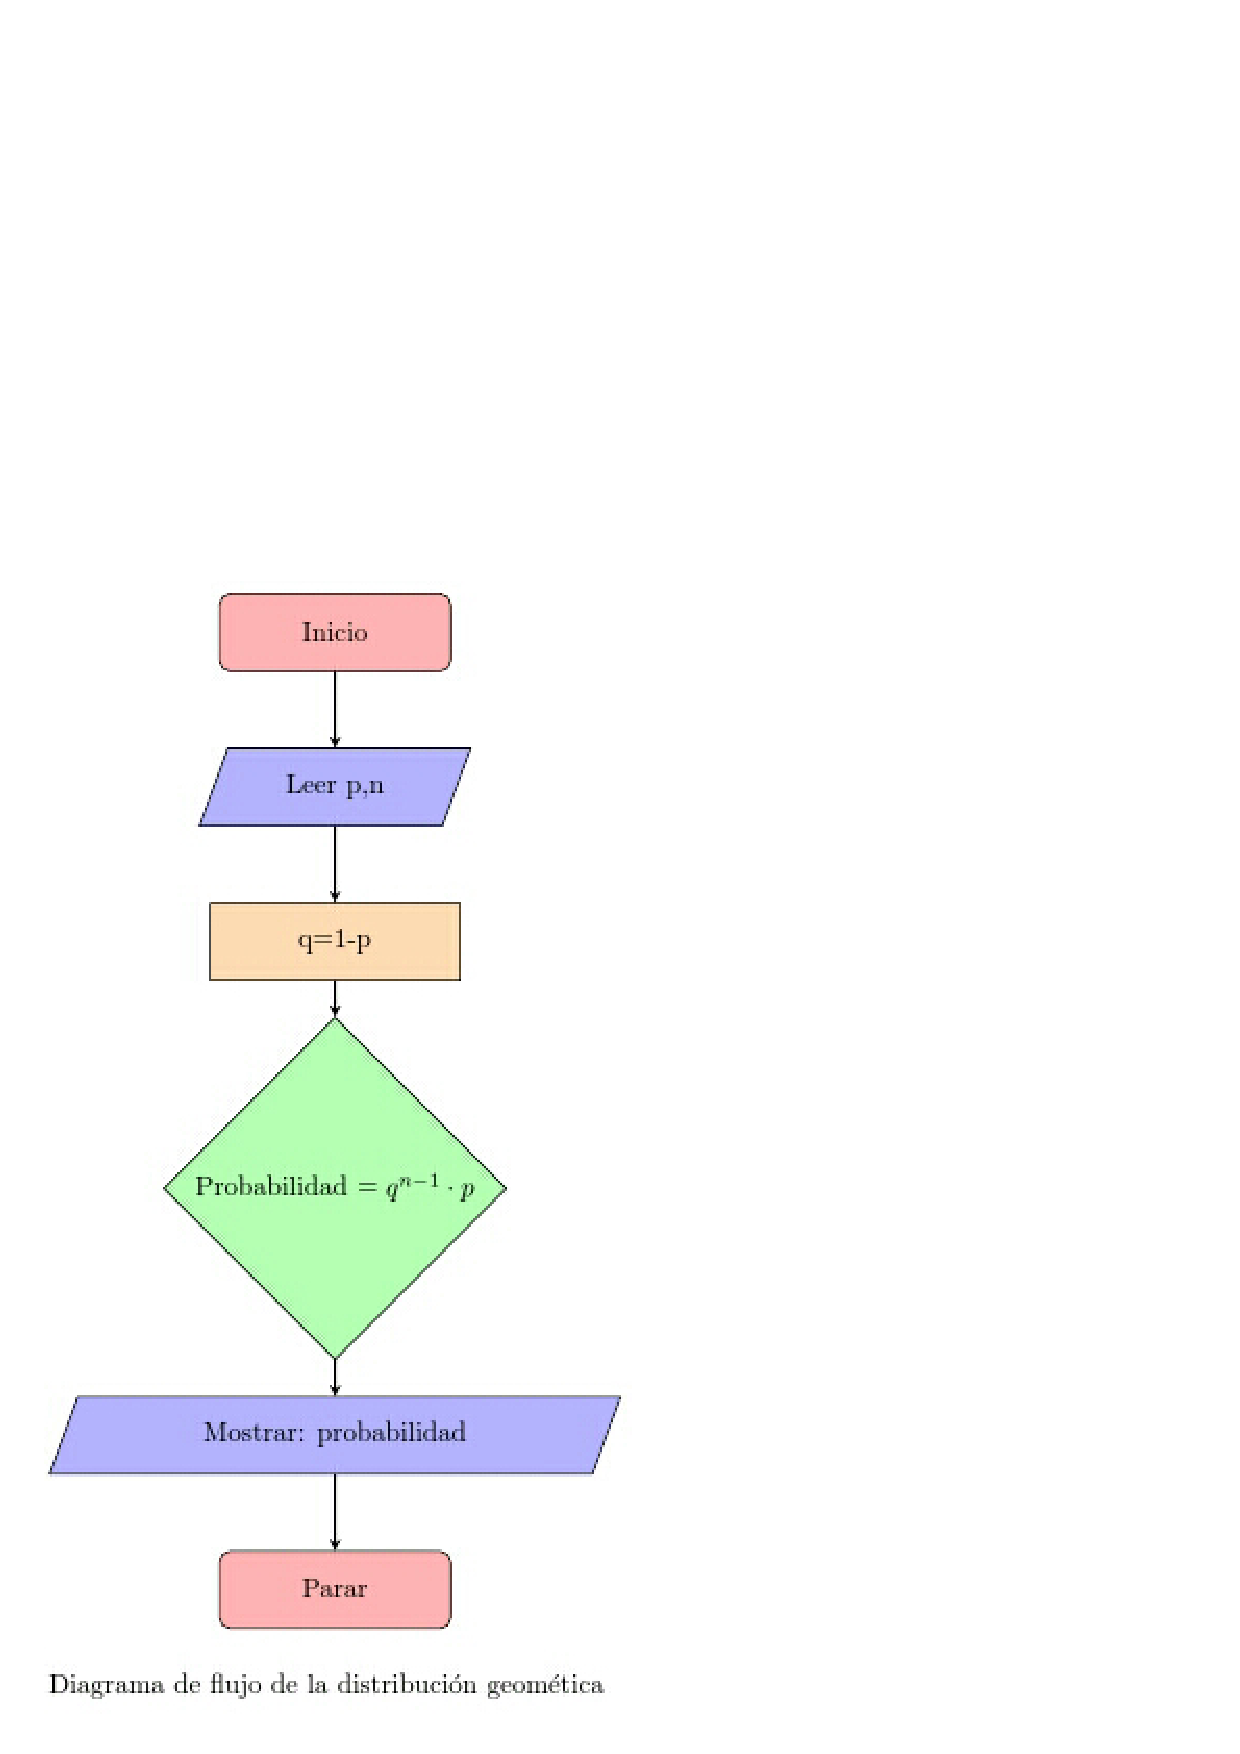
\includegraphics[width=5cm]{images/diafluj.png}
  \caption{Diagrama de Flujo de la Distribuci�n Geom�trica}\label{dflu}
\end{figure}	
  \item[Codifici�n] Vease el c�digo en  en el ap�ndice 1.
\end{description}
\end{enumerate}



%++++++++++++++++++++++++++++++++++++++++++++++++++++++++++++++++++++++++++++++
\section{Descripci�n del material}
\label{3:sec:2}
Tanto para la ejecuci�n en Python, como para la implementaci�n en \LaTeX{}, hemos utilizado:

\begin{enumerate}
	 \item \textbf{Ordenadores:}
%------------------------------------------------------------------------------
\begin{table}[!ht]
\begin{center}
		\begin{tabular}{|c||c|c|}
          \hline
          % after \\: \hline or \cline{col1-col2} \cline{col3-col4} ...
          Marca: & Modelo: & Procesador: \\ \hline
          Acer & Aspire 5735Z & 2.0 Ghz \\ \hline
        \end{tabular}
\end{center}
        \caption{Modelos de ordenadores y procesadores:}
        \label{marca:1}
\end{table}
        

%------------------------------------------------------------------------------


  \item \textbf{Versi�n de Python:}
  Para la realizaci�n del programa que soluciona los distintos problemas, anteriormente descritos, utilizaremos la siguiente versi�n de Python:
  \begin{center}
  \textbf{PYTHON 2.7.3 [GCC 4.6.3] ON LINUX2}
  \end{center}

  \item \textbf{Versiones de \LaTeX{}}
  As� mismo hemos utilizado las siguientes versiones de \LaTeX{} y distintos entornos de trabajo:\footnote{Ambos entornos, trabajan en el sistema operativo Windos (en sus distintas versiones, dadas en el cuadro \ref{marca:2})}
%------------------------------------------------------------------------------
\begin{table}[!ht]
\begin{center}

		\begin{tabular}{|c||c||}
          \hline
          % after \\: \hline or \cline{col1-col2} \cline{col3-col4} ...
          \rowcolor[RGB]{0,88,147} Version Miktex: &  Editor texto: \\ \hline\hline
           2.9 & TexMaker   \\ \hline
         2.9 & WinEdt 8.0    \\ \hline
        \end{tabular}

\end{center}
        \caption{Versiones de \LaTeX{}}
        \label{marca:1}
\end{table} 
%------------------------------------------------------------------------------



\end{enumerate}


%++++++++++++++++++++++++++++++++++++++++++++++++++++++++++++++++++++++++++++++
\newpage
\section{Resultados obtenidos:}
\label{3:sec:3}

Para la realizaci�n de la siguiente tabla \ref{tab:1}, nos hemos ayudado de los problemas resueltos en el cap�tulo 1. Se ha a�adido el c�lculo del error entre los resultados obtenidos, por el programa dise�ado en Python, en comparaci�n con los resultados obtenidos : ''a mano'' y con una calculadora online \cite{URL:XML}

%------------------------------------------------------------------------------
\input{tables/table.tex}
%------------------------------------------------------------------------------

%parrafo del tiempo

Tabla del tiempo:





%------------------------------------------------------------------------------
\begin{table}[H]
\begin{center}
\scalebox{0.6}{
\begin{tabular}{|c|l|l|c|}
\hline
\rowcolor[RGB]{0,88,147} \textbf{Problemas:  } & \textbf{p:} &\textbf{Tipo de problemas:} & \textbf{Tiempo de ejecuci\'on: } \\ \hline
 1 & 0.5 & $P(X\geq 2)$ & 0.000047 \\
 2 & 0.8 & $P(X=1)$ & 0.000007 \\
   & 0.8 & $P(X=2)$ & 0.000035\\
   & 0.8 & $P(X=3)$ & 0.000035\\
   & 0.8 & $P(X=4)$ & 0.000035\\
   & 0.8 & $P(X=5)$ & 0.000048\\
   & 0.8 & $P(X\leq 5)$ & 0.000045 \\
 3 & 0.16666666 & $P(X=3)$ & 0.000035\\
 4 & 0.4 & $P(X<3)$ & 0.000044\\
 \hline
\end{tabular}
}
\end{center}
\caption{Tabla del c\'alculo del tiempo.}
 \label{time}
\end{table} 
%------------------------------------------------------------------------------

% parrafo de la grafica

%------------------------------------------------------------------------------
\begin{figure}[!th]
\begin{center}
\includegraphics[width=0.7\textwidth]{images/figura1.png}
\caption{Ejemplo de figura}
\label{fig:1}
\end{center}
\end{figure}
%------------------------------------------------------------------------------




%++++++++++++++++++++++++++++++++++++++++++++++++++++++++++++++++++++++++++++++
\section{An�lisis de los resultados}
\label{3:sec:4}

bla, bla, etc.

